\chapter{Тельбин}

Поговорим теперь про озеро Долобское, пролив Долбичку, озеро Тельбин и связь всего этого с летописной речкой Золочей.

Эту головоломку решают уже несколько сотен лет, рассматривая задачу лишь на узком отрезке времени и пространства, поэтому приходят к противоречивым выводам, которые легко поколебать, добавив в рассуждения упущенный из виду довод.

В нашем же повествовании местом действия послужит весь левый берег, временем действия – сотни лет, а действующие лица будут появляться по мере надобности.

Современный пролив Долбичка. Черторыя около Труханова острова разделяется на два рукава. Один идет прямо, другой выгибается к востоку. Остров между рукавами на современных картах называют Долобецким (в конце 19 века его северная половина была отдельным островом Кутом). Туда перебираются небольшим мостом с Гидропарка. А пляж нудистов «Долбичка» лежит напротив, на юге Труханова, тоже омываемый проливом Долбичкой, с юго-восточной стороны. Берег пляжа в первой половине 20 века был частью суши Гидропарка.

Прямое русло Долбички и служит сейчас основным руслом Черторыи, ибо идет прямо, по виду естественно продолжая реку, в то время как восточный рукав выглядит второстепенным. Но если следовать взглядом на юг, то именно восточный рукав продолжается в качестве Русановского пролива, а вот Долбичка через Венецианский пролив упирается в северный берег Гидропарка, напротив пляжа нудистов.

От прежней Долбички остается только название, протяженность между широтами, да направление течения, и то – с середины 19 века оно сменилось с юго-западного на южное. Веками русло плясало, извиваясь по местности, на нее влияли как природные, так и человеческие силы – рылись каналы, сооружались запруды. И если только за прошедшие полтора столетия русло изменилось совершенно, то как заглянуть в более далекое прошлое?
%Русло Долбички начала 21 века пересекается по координатам с руслом Долбички середины 19 века только на двух коротких отрезках. На нее влияли как природные, так и человеческие силы – рылись каналы, сооружались запруды. 

А ведь считается, что «на месте Долбички» раньше находилось Долобецкое озеро, упоминаемое в летописях и старинных земельных документах. Да где на месте, на каком? Русло Долбички какого времени принимать за «это место»?

В летописи единожды упомянуто «озеро Дулебское» и несколько раз просто урочище «Долобьске». Там князья иногда сходились на совещания. Например, в 1103 и 1111 годах Святополк и Владимир встречаются в шатре «на Долобьске», причем не указано, озеро это или такая местность. А в 1101 году князья-братья собираются на Золочи.

Долобское озеро вписано в Жалованную грамоту Киевского воеводы Юрия Монтовтовича Пустынно-Никола\-евскому монастырю, 4 июля 1508 года:

\begin{quotation}
Я, Юрьи Михайлович Монтовтовича, воевода Киевский, державца Черниговский и Любецкий. Били нам челом старци з монастыря Святого Николы Пустыньского, штобыхмо придали на тот монастырь и церкви Святого Николы озеро, на имя Долобеск, и с устьем в острове в Туханове.
\end{quotation}

Вообще сведения о Долобском озере скудны. В путеводителе по Киеву конца 19 века впрочем говорится о Долобском как об озере на Труханове, и что оно летом часто пересыхает. Но возможно, сочинитель принимал за Долобское озеро другой водоем.

Долобское озеро (а озером тогда могли называть и залив) и Золоча возникают в летописи при описании попыток Гюрги (Юрия Долгорукого) в 1151 году форсировать Днепр, чтобы выбить Изяслава из Киева. Наиболее подробно сие описано в Ипатьевской летописи:

\begin{quotation}
И поиде Гюрги к Киеву\footnote{Гюрги плыл на лодках по Десне из Городка Остёрского.} и сташа в Родуни, и придоша Половци диции\footnote{Дикие.} мнози Дюргеви в помочь; и Изяславу же блюдущу вбрести в Днепр, и тако начаша ся бити по Днепру у насадех\footnote{Насад – речное судно, у которого основа долбленая, а борта набиты, досками.} от Кыева оли и до устья Десны, ови ис Киева в насадех выездяху биться, а они ис товар; и тако бьяхутся крепко, не могоша бо что успети противу Киеву. 

Бе бо исхитрил Изяслав лодьи дивно: беша бо в них гребци невидимо, токмо весла видити, а человек бяшет не видити; бяхуть бо лодьи покрыты досками, и борци стояще горе в бронях\footnote{Бойцы стояли наверху лодок, одетые в броню.} и стреляюще, а корменика два беста, един на носе, а другый на корме, а может хотяхуть, тамо поидяхуть, не обращающе лодий\footnote{Два рулевых, на носу и корме, что позволило плыть в любую сторону и поворачивать, не делая разворот лодьи.}.

И оттоле Гюрги сгадав с Володимером с Давыдовичем, и с Святославом Олговичем, и с Всеволодичем Святославом, и с Половци, и хотящим вниз пойти к Витечевьскому броду, не смеющим же им пустити лодии мимо Киев, но пустиша е во озеро Дулебское и оттоле волочиша е берегом в Золотчу, по Золотчи же внидоша во Днепр лодье их; Половци же Гюргеви идяху по лугу.
\end{quotation}

Гюрги в лодьях из Десны смог «сташа в Родуни». Про Родунь мы будем рассуждать в других главах, пока примем, что это некое урочище близ устья Десны. Однако мы не знаем, где было устье Десны в летописное время, посему передвижения Гюрги начинают проясняться только у Труханова острова.

На помощь Гюрги, к Родуни, прибывают дикие Половцы. Но Изяслав, стерегущий (блюдущий) брод через Днепр, не дает Гюрги и Половцам переправиться. Изяслав сражается в насадах, а у Гюрги есть лодьи и военный обоз, повозки. Фронт разворачивается по Днепру от Киева и до устья Десны. Изяслав и дополнительные насады из Киева мешают Гюрги.

%Поскольку речь идет о седой старине, уместно предположить, что устье Десны могло быть где угодно – а хоть бы Десной считалось и русло в протяженности современных Десенки и Черторыи, и тогда устье Десны вполне подходило к Труханову острову, а не к Муромцу, как нынче.

%Вот незадача. Для простоты рассуждений поступим как делают ученые. Примем, без всяких доводов, что устье Десны лежало примерно на той же широте, что и сейчас. Я вообще дальше буду с натяжкой делать некоторые утверждения, допуская, что русла с летописных времен изменились не сильно – что, конечно же, маловероятно.

Гюрги держит совет с Володимером Давыдовичем, Святославом Олговичем, Святославом Всеволодичем, и Половцами. Здесь перебраться на правый берег не получается, что делать? Искать другое место. Решают пробиваться вниз к Витичевьскому броду\footnote{Возле селения Витачов (Вытачов) близ Триполья. У южной околицы Витачова, над Днепром, есть древнее городище, возможно то самое, о котором пишет Константин Багрянородный в «Об управлении империей», говоря о судоходстве и том, что Росы от крепости Киоавы «двигаясь по реке Днепр, они спускаются в Витичеву, которая является крепостью-пактиотом Росов».}. Брод нужен для обоза Половцев. По какой-то причине Гюрги не смог сразу плыть вниз по Днепру, и пускает свои лодьи в озеро Дулебское, оттуда волочит их по берегу в Золочу, а из Золочи лодьями выплывает в Днепр. Половцы же едут лугом, параллельно лодьям.

Будучи в Днепре, Гюрги вводит свои лодьи в Дулебское озеро. Значит, оно было заливом, соединенным с Днепром!

Совершенно верно. А рядом, западнее, протекал рукав Днепра, ставший потом Матвеевским заливом. Во время Гюрги это был, думаю, основной рукав Днепра, где и разворачивалось сражение. Черторыя не упомянута – вероятно, она еще не существовала.

%И привычная нам Черторыя в то время просто не существовала и не доходила руслом к Долобскому «озеру», а точнее заливу.

Затем Гюрги перетаскивает лодьи по суше из Дулебского озера в Золочу, а из Золочи уже выплывает в Днепр, ниже по течению. Следовательно, Золоча впадала в Днепр, а между нею и Дулебским озером была суша. Это также означает, что никакой другой воды в то описываемое время между Золочей и Дулебским озером не было. Важно!

Летописец очень тщательно передает последовательность перемещений войск. В Дулебское озеро из Днепра лодьи не перетаскивали, а из Дулебского в Золочу – понадобилось волочить по суше. Это однозначно говорит о том, что Дулебское – залив, а Золоча – река или другой залив, тоже соединенный с Днепром. И между Дулебским заливом и Золочей был отрезок суши. Выстраивается цепочка с севера на юг: Днепр – Дулебское – суша – Золоча – Днепр.

%Отсюда следует, что в рассматриваемой местности не просто не существовало Черторыи, но и другого рукава Десны, если только под Десной не подразумевалось русло Черторыи. Иначе, будь отдельный рукав, Гюрги в своих перемещениях из Долобского в Золочу неизбежно должен был его пересечь. Этого не случилось.

%Если бы какое-то русло, рукав Десны, будь то Десенка или Черторыя, протекало так (от Десны до Гидропарка) при Гюрги, то Гюрги в своих перемещениях из Долобского в Золочу неизбежно должен был пересечь Черторыю. Этого не случилось.


%Значит, Черторыя тогда вероятно не существовала как поименованный водоток от Десны, и уж точно не доходила до широты озера Долобского. Ибо позже таки дошла и течет теперь по месту озера Долобского как пролив Долбичка.

%Либо значит, что Десной таки считалось русло в протяженности нынешней Черторыи, однако по ряду причин мне неудобно так думать.

Попади мы в летописное прошлое, то очень удивились бы, увидав, как всё было на деле. Но судить можем лишь по более новым картам.

Рассмотрим кусок плана 1750 года. Верхняя сторона карты – запад.

\begin{center}
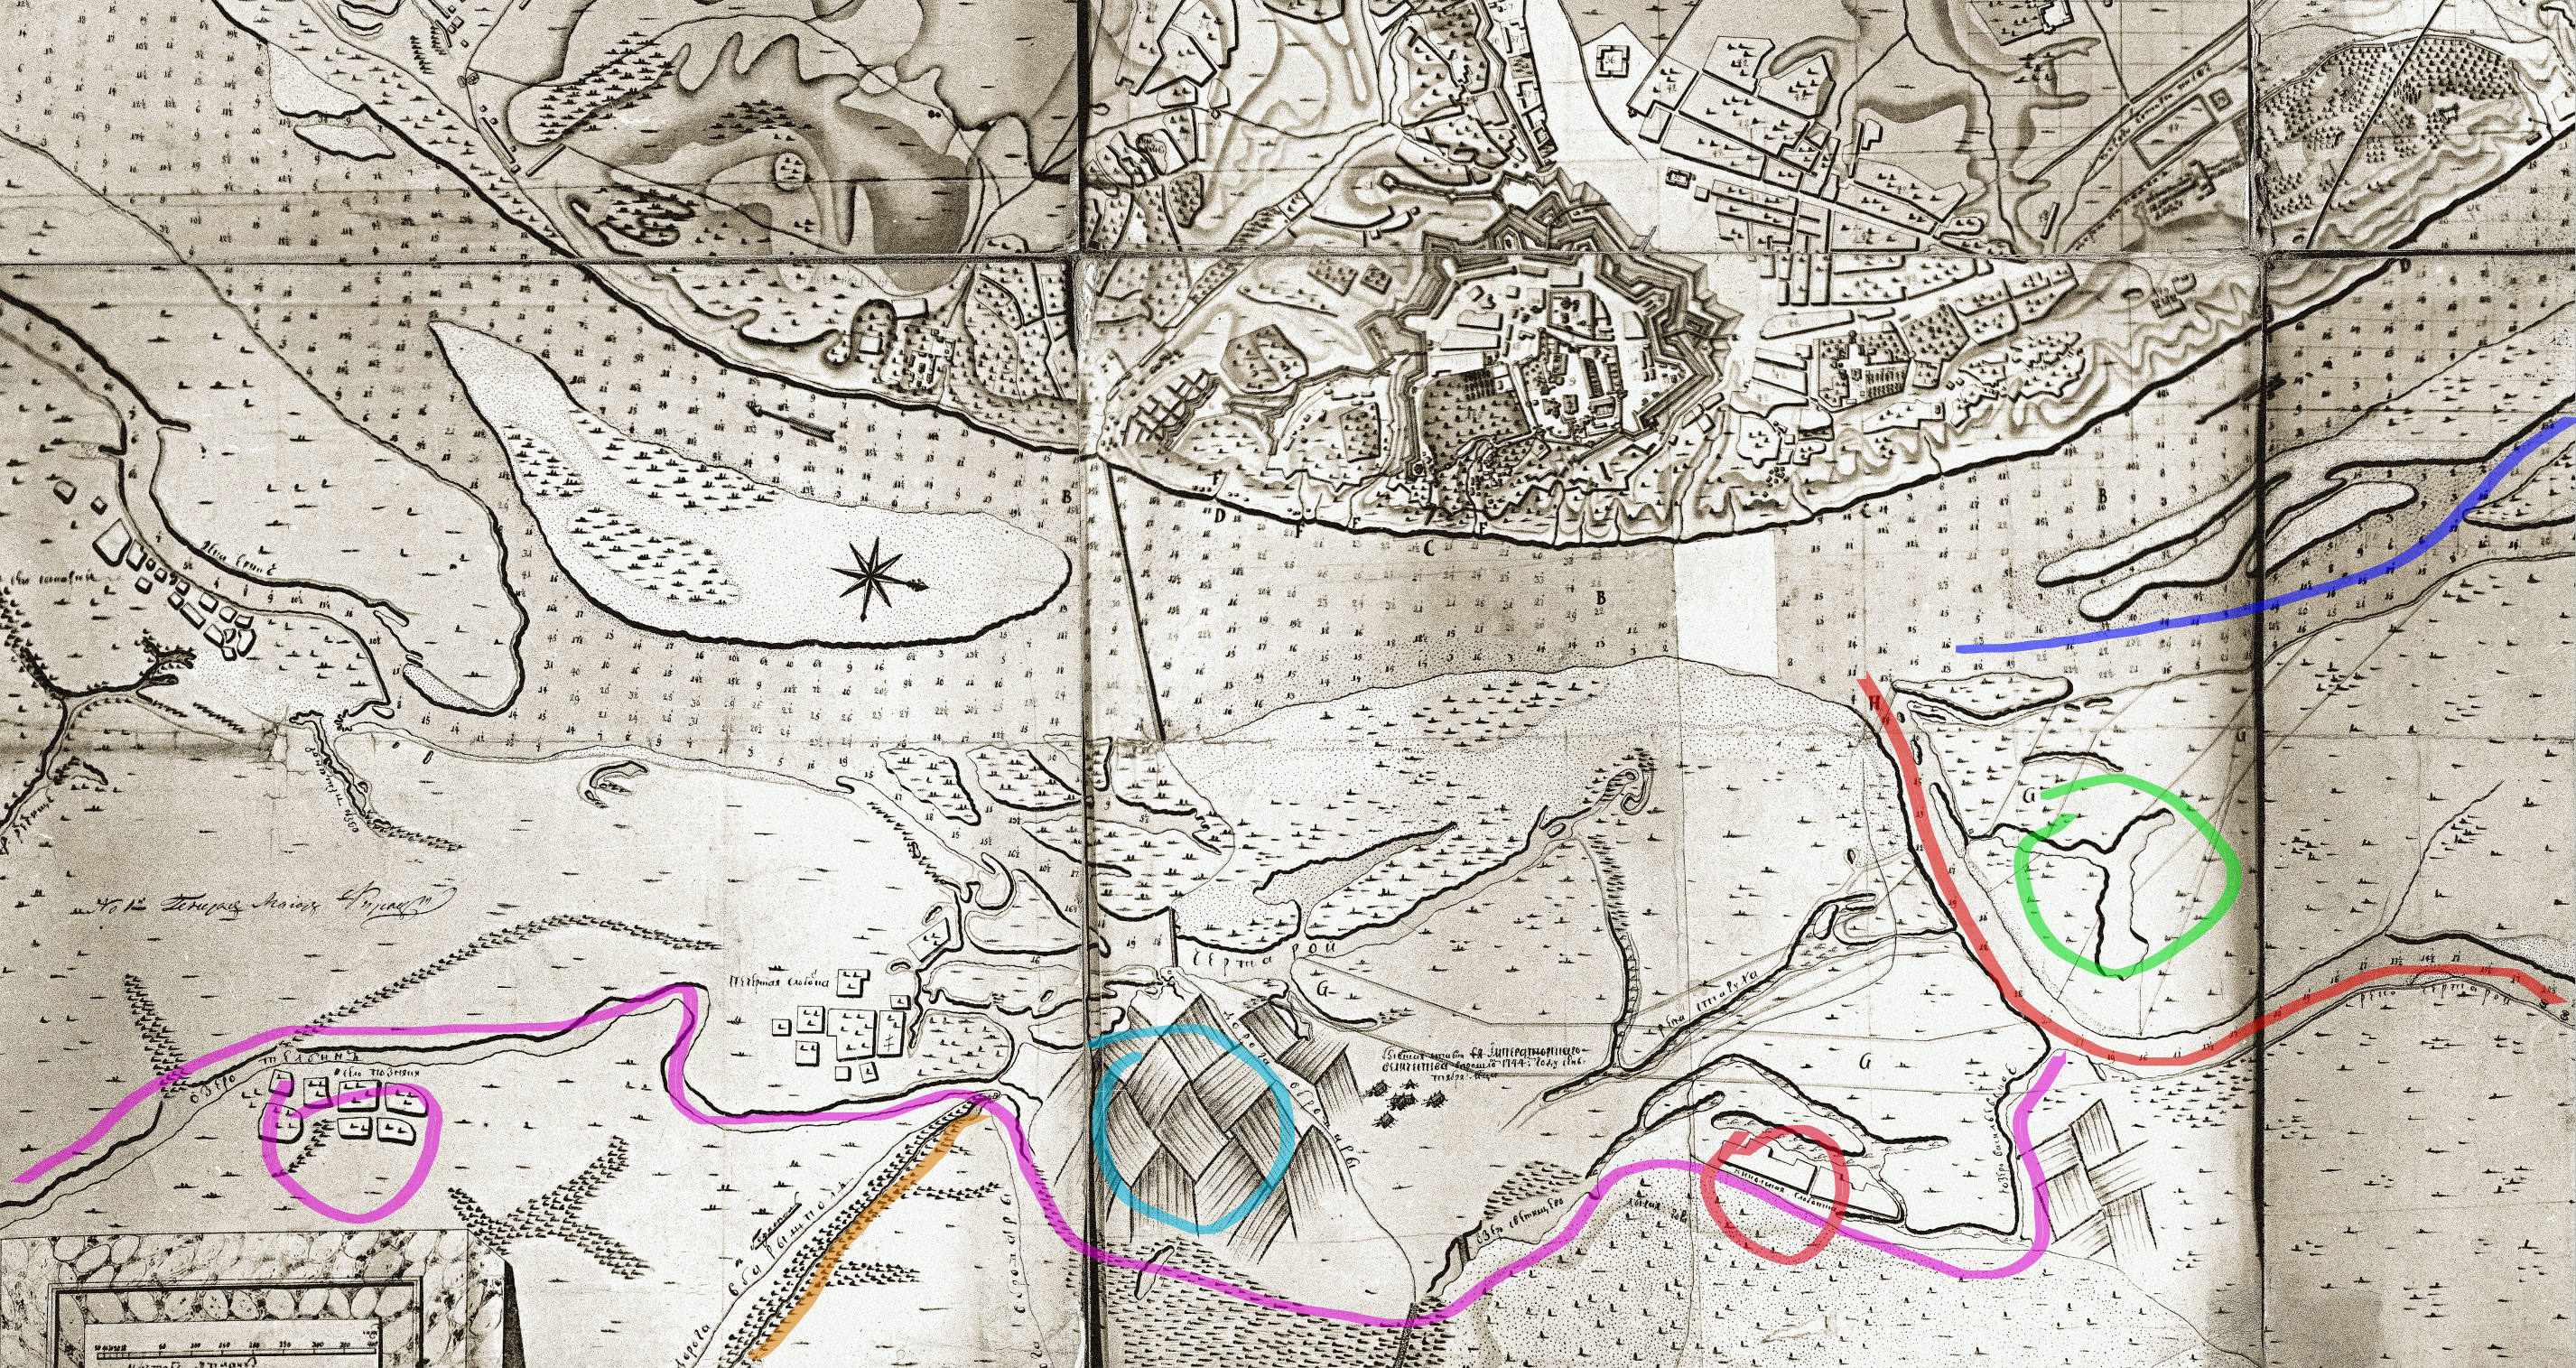
\includegraphics[width=\linewidth]{chast-gorodki/terbin/1750-telbin-new.jpg}
\end{center}

%На куске плане 1750 года видно положение, где основное русло Черторыи (подпись «река Чертарой», правее, не поместилась) сворачивает к Днепру на широте эдак моста Метро, а южнее, хотя и подписан там залив «Чертарой», очевидно, что это не продолжение Черторыи, но порождение Днепра. Рассмотрим внимательно. Верхняя сторона карты – запад.

Подобный шестеренке многоугольник посередине вверху – крепость вокруг Лавры. Вертикальная линия через Днепр в первой трети картинки – переправа около Наводничей. Это главные ориентиры.

Салатовым кружочком я обвел Долобское озеро. Точнее, на картах 19 века в том месте находится водоем других очертаний, подписанный как Долобское озеро.

Красный кружок – Никольская слободка.

Голубой кружок – вспаханные поля, где ныне Русановка.

Малиновый кружок – село Позняки.

Красной линией показано основное русло Черторыи (подпись на карте, «река Чертарой» – есть, однако не поместилась на скопированный мною кусок). Слева (южнее) от него теперь мост Метро. 

Еще южнее лежит «река Старуха», а потом снова «Чертарой», южнее Никольской слободки. По виду он похож, скорее, на старицу Днепра. Через него перекинут мост от дороги с Наводницкого моста. 

Синяя черта – рукав Днепра, ставший потом Матвеевской затокой.

Оранжевая черта – речка Дарница.

Малиновая линия – так я предполагаю некогда единое русло-продолжение Долобецкого залива. В районе Никольской слободки я отвел его чуть ниже настоящих водоемов. На 1750 год русло включает в себя озеро Васильевское, Русановское, Светищево, и болото переходящее в речку Тельбин.
 
Что получается? 

Если Гюрги в 1151 года плыл по «синему» руслу Днепра, то на восток (на карте – вниз) от этого русла Днепра лежал залив, ставший потом Долобским озером. В его северную часть можно было зайти из основного русла. Чем Гюрги и воспользоваться, чтоб укрыться от неприятеля.

Как далеко простирался залив в сторону Золочи?

Долобское озеро на карте 1750 года словно пересекается «красным» руслом Черторыи. А что к востоку, на карте – ниже этого пересечения? А там продолжается сей прежний Долобский залив. Пока Черторыя не перерубила залив надвое, либо разделение произошло по другой причине, это было единое русло. И дальше оно продолжается на юг, в обход современной Русановки с востока. 

На Светищево и это болото да истоки озера Тельбин (образца середины 19 века) почти совершенно накладывается нынешний Русановский канал.

Печерская слободка на этом плане то же, что на других – Кухмистерская слободка. Она лежала по западному берегу Тельбина, между ним и Днепром. А на восток от Тельбина позже возник хутор Зательбин Березняк. Позже на месте обоих селений был построен жилой район Березняки.

% с Печерской слободкой на карте петрушка получается. Дореволюционные карты так именуют два разных поселения. Одни карты обозначают так местность, известную ныне как Гидропарк. Другие же Гидропарк называют Предмостной слободкой, а Печерской слободкой – хутор Зательбин Березняк, он же Березник, где позже возник жилой массив Березняки.

%Дореволюционные планы частенько величают Предмостную Слободку – Печерской. 

%На карте же 1750 года, умозрительно, находясь примерно на широтах между Наводничами и Выдубицким монастырем, эта Печерская слободка однозначно сопоставляется с Кухмистерской с тех же позднейших карт.

На плане Сноевского, «речка Тельбин» – а ныне от нее известен отрезок в образе озера Тельбин – отождествлена с летописной Золочей. Верно ли?

Берлинский предполагал подобное, не называя впрочем «Тельбин», но ясно указывая на левобережные водоемы напротив Наводничей. Многие современные исследователи вообще притягивают исток Золочи чуть не на Труханов.

Такое понимание основано на представлении, что Долобское – обыкновенное озеро на Труханове, а не залив, имеющий большую протяженность с севера на юг. В этом упрощенном представлении в самом деле, лучшего кандидата на роль Золочи, чем речка Тельбин, не найти.

Но по моим прикидкам, Тельбин – это продолжение Долобецкого озера-залива, как я отметил малиновым на карте 1750 года, где, по тогдашним представлениям, «озеро Тельбин» подписано рядом с Позняками.

В более ранних земельных документах, различались речка Тельбин и одноименное озеро. По карте 1750 года видно, что южнее современной Русановки, Тельбин составляется из: потока из болота, огибающего Русановку; речки Дарницы; наконец туда попадает вода из лабиринта днепровских заливов.

Возьмем старое название Тельбина, которое я вычитал в каком-то земельном документе. Толбин\footnote{Мост «у Толбина», за Днепром, принадлежал в 17 веке Выдубицкому монастырю, что заведовал паромной переправой от устья Лыбеди к Осокоркам. Надо думать, что и мост через Толбин находился там же.}. Попробуйте на слух отличить «Толбин» от «Долбин». Буквы «д» и «т» гуляют, взаимозаменяемы. Толбин то же, что Долбин, а значит... Между урочищем Долобским, Долобским озером и Долбином прямая связь! Не только по названию, но и по смежности мест и остаткам единого русла, прослеживаемых на карте.

Тельбин-Долбин это продолжение Долобского залива. Некогда единое русло, пересеченное потом Черторыей в районе моста Метро. До такого изменения местности, Долбин был длинным заливом Днепра, даже рукавом, поэтому-то Гюрги и мог плыть сначала по нему, а затем перетащить лодьи в «Золочу».

%Обратите внимание на острова напротив Наводничей. Почему там острова? Потому что обмеление. Почему обмеление?

%Вспомним Почайну. Мели возникали там, где впадали притоки. Выше мели раздувалось русло. Образование обходных рукавов. И островов между ними.

%Внизу, посередине карты, что за речка с лесистыми берегами ползет вверх (на запад)? А это речка Дарница впадает в Долбин. Вот вам и ответ, почему обмеление и острова. Не забудем и о влиянии Черторыи.

Тельбин скупо отражен в земельных документах и больше на картах. В грамоте 1694 года царей Иоанна и Петра Алексеевичей, подтверждающей Киево-Братскому монастырю права на земли и угодья, сказано кроме прочего про сеножать Подкурье, границы которой связаны с Тельбином:

\begin{quotation}
село Позняки [...]

Другая сеножать Подкурье по дальнюю гать рубежем, почав от озера Тербина жерелом Дарницею до нижней мельницы Печерской, до Воскресенщины, от мельницы убедью до Острого Рога, а от Острого Рога до Шаломин, тою убедью, от Шаломин в конец Урлева гради, от Урлева в Пенные лозы, а от Пенных лоз в Довгушку озеро, из Довгушки жерелом в Серебренный-Кол, от Сребренного Кола длиной малою, в конец Вязок, в Княжей Затон, от Княжего Затону на брод под Троецкий футор, от брода жерелом до Весняка речки, Весняком до Синятина, от Синятина до Порубежнаго, от Порубежнаго до Телячева, от Телячева, речкою Позняковкую, до моста на Тербин речке, да в речку Дарницу.
\end{quotation}

Сейчас на Позняках есть улицы Княжий затон, Урловская, Срибнокильская. Мне впрочем неизвестно, насколько соответствует положение этих улиц упомянутым урочищам.

Кроме уймы других названий, которые и не отыщешь уже на местности, из грамоты можно заключить важное – в Тельбин впадает речка Дарница (как и поныне, только в другом месте), и через Тельбин был мост, а значит проходила дорога. Кроме того, в грамоте различаются речка Тербин и озеро Тербин. Понимаю это так – было русло с текучей водой, и отрезанная от нее часть со стоячей. Не про Долобецкое ли озеро говорится?

Рельеф левого берега сильно изменился и я предпочитаю в качестве ориентира использовать неизменные правобережные Наводничи, так что проведя оттуда линию, получаем, по плану 1750 года, что устье Дарницы было в верхней части Тельбина, севернее нынешнего озера Тельбин, а не в современном озере Нижний Тельбин. Сейчас ведь иначе – Дарница ровным каналом отведена в Нижний Тельбин, а оттуда идет слив по коллектору в Днепр.

%На плане 1843 года полковника фон Руге, Тельбин уже не залив Днепра – между истоком и Днепром есть суша к югу от будущего Броварского шоссе. Тельбин на этом плане занимает часть нынешней Русановки, Березняков.

%, и – опять-таки на широте Неводничей в него впадает ручей, исходящий из похожего на крючок водоема. Это отрезок Дарницы, вытекающий из Дарницкого озера.

\begin{center}
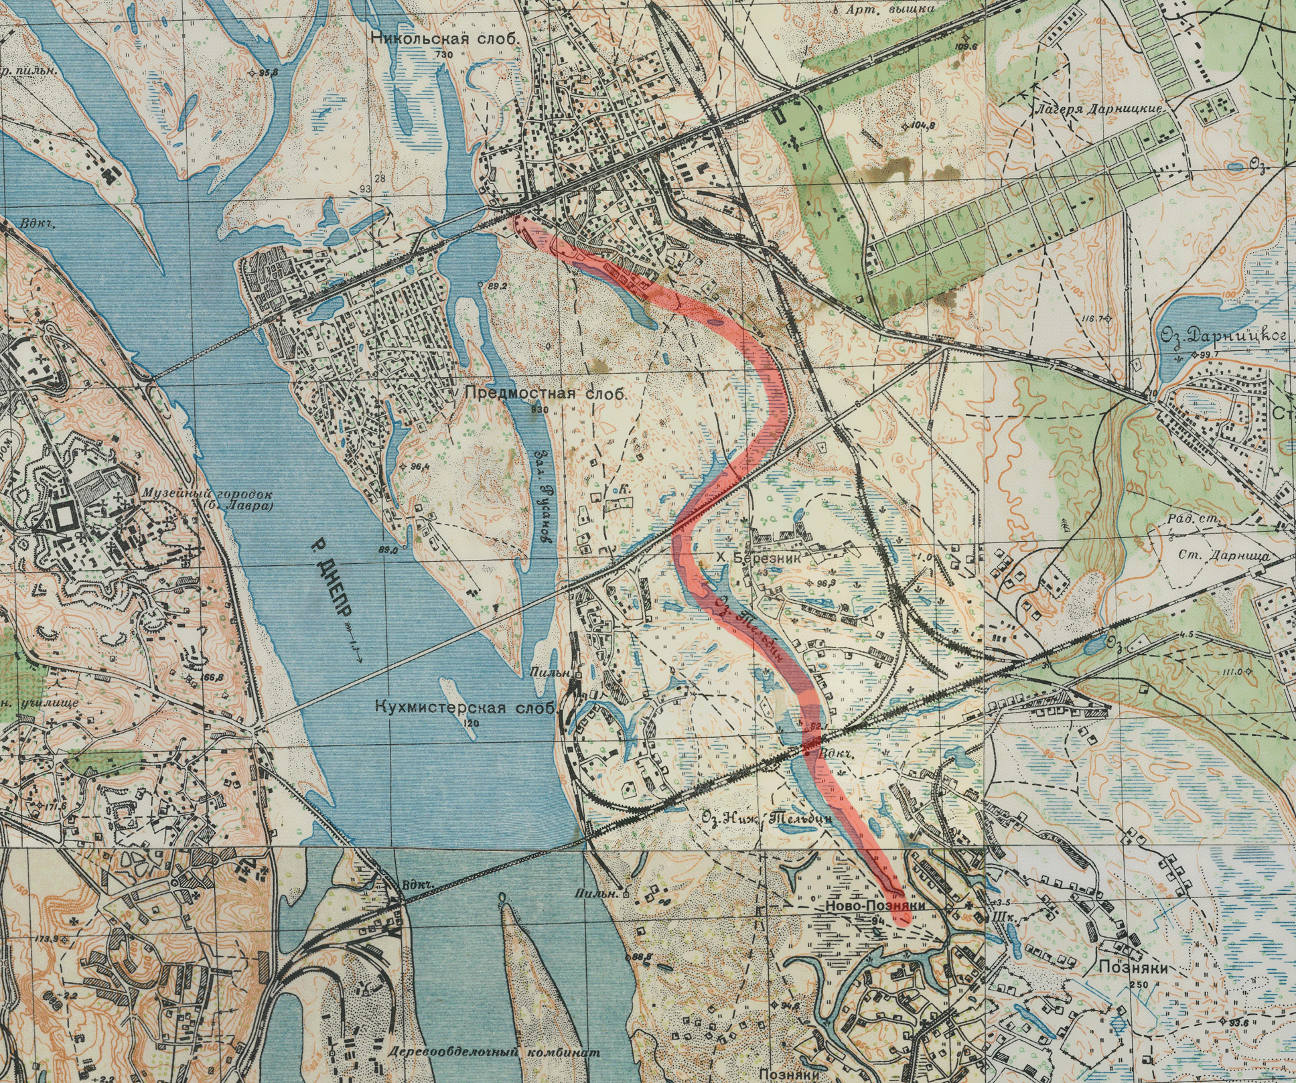
\includegraphics[width=\linewidth]{chast-gorodki/terbin/rkka-telbin-s.jpg}

\textit{На карте РККА 1930-х, красной линией я отметил остатки всего русла Тельбина-Долбина начиная от Никольской слободки.}
\end{center}

С речкой Дарницей мы будем разбираться позже, с ней тоже много вопросов. На карте Шуберта уже середины 19 века устье Дарницы – а речь идет об отрезке Дарницы, что вытекал из одноименного озера – теряется в безмерном болоте около хутора Позняки, примерно в окрестностях современного озера Горячки.

Постепенно русло Тельбина дробилось – его перерубали разные гати для прокладывания по ним дорог, а также влияли естественные причины.

Во второй половине 19 века всё к востоку от Тельбина заболачивается до Старой Дарницы.
Болото возникает и вокруг озера Дарницы – да и речка Дарница представляет в то время перетекающие друг в друга болота.

В 1860-х поперек Тельбина надо было проложить рельсы Киево-Курской железной дороги\footnote{С 1891 года переименованной в Киево-Воронежскую железную дорогу. Годы открытия участков: 1870 – от Киева до Днепровского моста; 1869 – от Днепровского моста до станции Бровары, и так далее. Чуть южнее взорванного 19 сентября 1941 г. Днепровского моста в 1949-м построили Дарницкий железнодорожный. От Днепровского моста осталось несколько опор.}. Для этого соорудили насыпь, и Тельбин распался на просто Тельбин и Нижний Тельбин. Речь идет о железной дороге, что теперь проложена через Дарницкий мост и шурует мимо Березняков к вокзалу «Дарница». Насыпь с железной дорогой поныне высится по левому берегу.

Между Тельбином и Днепром оказалось зажатой Кухмистерская слобода, что занимала нынешний квартал, ограниченный улицами Тычины, Шумского, Березняковской и Днепровской набережной. Со стороны озера на нее наползало болото – ведь после преграждения озера дамбой, вода стала накапливаться вдоль нее.

Положение исправилось позже, когда речку Дарницу направили в другое русло с выводом южнее железной дороги, в Нижний Тельбин. 

%А остатки прежнего русла ее, которое подходило к Тельбину в верхнем его течении, и поныне сохранились под именем болота Серой цапли\footnote{50°25′40″N, 30°37′13″E.} около железной дороги между заводом Фанерных плит с северо-востока и чудовищным массивом гаражей с запада. Там же начинается улица академика Шлихтера, и от железной дороги, что идет с востока на запад, отделяется еще одна ветка на север, вдоль Шлихтера (на ряде карт 2014 года ее успели раздробить на улицы Мартовскую и Вифлеемскую) и к Левобережной.

В начале 20 века русла обоих Тельбинов, простого и Нижнего, хоть и разделенные, еще сохраняли вид луговой реки. На картах они обозначались пока единым озером, доходящим до Позняков и сворачивающим у поселка в сторону Днепра. 

Но уже к 1914 году Нижний Тельбин укоротился около северной границы Позняков и на карте того года подписан «оз. Коростышево», либо такое название относится к соседнему с запада водоему. 

К востоку же от этого вытянутого с севера на юг Нижнего Тельбина было озеро Ольхово (любопытно, где ставить ударение?). Вероятно следы его – водоем близ перекрестка Ивана Кочерги и Григоренко. А остаток прежнего Нижнего Тельбина – озеро Королек между улицами Канальной и Здолбуновской, около завода высокоточной аппаратуры «Буревестник», основанного в 1967 году и работавшего тогда на оборонку.

Современный Нижний Тельбин – образование искусственное, просто широкий канал, на месте которого еще в середине 20 века был бугристый пустырь.

Посмотрим на аэрофотоснимок 1943 года:

\begin{center}
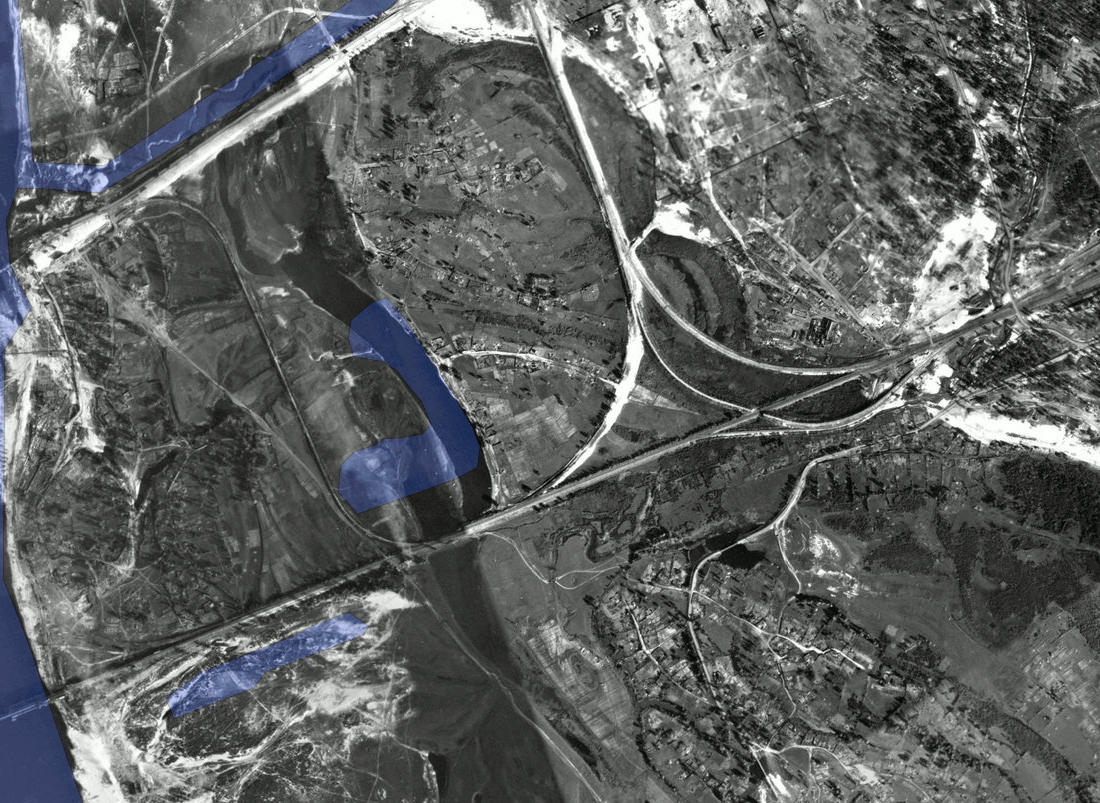
\includegraphics[width=\linewidth]{chast-gorodki/terbin/s_telbin-1943.jpg}
\end{center}

Синим цветом я отметил современный рельеф. Слева – Днепр, в верхней левой части наискось – Русановский канал вдоль современного проспекта Воссоединения. Большое синее пятно загогулиной – озеро Тельбин, синяя горизонтальная сопля – Нижний Тельбин. И сопоставьте с Тельбином за 1943 год!

Вот он начинается на севере, у нынешнего моста около остановки «бульвар Давыдова», к западу от рынка. Истока не видно, на горло ему наступила насыпь с дорогой. Насыпь? Но ведь теперь ее нет! Верно. Ведь близлежащие районы – Березняки, Русановку – насып\'али, поднимали их уровень перед строительством жилмассивов. Прежде местность была ниже, а дорога, где сейчас проспект Воссоединения, проходила насыпью по болоту. И к северу от нее застрял исток Тельбина, мы видим его – вьется змейкой вдоль насыпи, выше ее, и в сторону Днепра.

Южнее насыпи Тельбин шел по теперешним дворам в квартале между улицами Серафимовича, Бучмы, Тычины. Дом по Бучмы, 8 – стоял на озере. Детский сад №577 – на озере. Тычины 9Б – на самом берегу. Школа №191 – прямо на озере.

Современное состояние Тельбина и Нижнего Тельбина.

В Нижний отведена речка Дарница и мутный, прорытый во второй половине 20 века поток, что выходит из земли около улицы Здолбуновской\footnote{Возле 50°25'10.76"N 30°37'41.46"E.}, и протекает мимо озера Прорвы, отделенный полоской суши. На берегах его виднеются развалины частных усадеб и впавшие в дикость сады по улице Любарской (перерубленной пополам проспектом Григоренко), где на 2014 год осталось немного позняковской старины. Можете посмотреть кадры оттуда в моем фильме «Озёра Прорва и Горячка».

Затем мутный поток уходит в коллектор у проспекта Григоренко\footnote{50°25'16.87"N 30°37'17.82"E}, где соединяется с речкой Дарницей, и общие воды выходят из коллектора в канал чуть севернее начала улицы Канальной, у перекрестка с Дарницким шоссе и проспектом Григоренко\footnote{50°25'26.1"N 30°37'5"E}. Прямой канал, прорытый в 1950-х, идет на запад и ныряет в трубы под мостом Сортировочной улицы, а потом на запад от нее вливается в водоем, слывущий ныне Нижним Тельбином.

На плане 1991 года видна несколько иная картина. Тонкая синяя линия от Тепловозной улицы до впадения в Нижний Тельбин под станцией «Левый берег» – это рукотворное, но поверхностное русло Дарницы. Там, где она впадает в озеро, теперь перекресток Дарницкого шоссе и проспекта Григоренко.

Шоссе еще не существовало, его проложили в 2011-12 годах при постройке «моста Кирпы»\footnote{Автомобильный мост, построен рядом с Дарницким железнодорожным, официально оба моста называют как один – Дарницкий.}, а до этого просто шла железная дорога безо всякого параллельного шоссе. На месте массивной станции «Левый берег», почти вокзала, была обычная полустаночная платформа. %Неподалеку, в восьмидесятых, вдоль Нижнего Тельбина на пустыре была дрессировочная площадка для собак.

В 1991-м Нижний Тельбин имел вид эдакой буквы «Г» с верхней палочкой в обратную сторону. Эта палочка и есть канал. А вертикальная палочка – старое, историческое русло. Вот его-то и не стало! Теперь оно застроено серой промзоной, лишь озеро Королек, тщательно загороженное от людей бетонными заборами, напоминает, куда дотекал Тельбин – но об этом никто не знает. 

\begin{center}
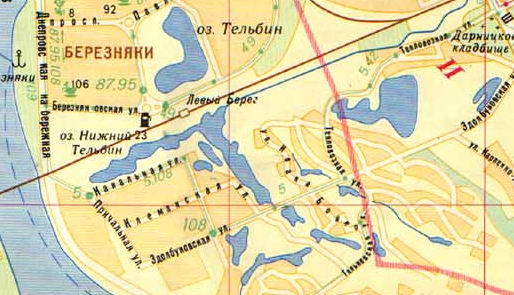
\includegraphics[width=\linewidth]{chast-gorodki/terbin/1991-telbin.jpg}

\textit{Фрагмент карты 1991 года.}
\end{center}

%На берегу Королька – завод высокоточной аппаратуры «Буревестник», основанный в 1967 году и работавший тогда на оборонку. На нем производились радиоэлектронные системы наблюдения для нужд флота. 

%В первом десятилетии 21 века «Буревестник» выпускал, кроме приборов того же рода, аппараты искуственной вентиляции легких, машинки для счета купюр, FM-приемники и другие товары. 

В ходе работ над мостом и прилегающим Дарницким шоссе, на протяжении от Фанерной улицы\footnote{На этой улице был поселок рабочих Фанерного завода. Посёлок сожгли немцы во время Великой Отечественной войны. Потом Фанерка отстроилась промзоной и жилыми домами.} речку Дарницу, где она выходит из коллектора, снова туда загнали, упаковали в бетонный короб – под асфальтом Дарницкого шоссе и до проспекта Григоренко!

Про канал. Еще до того, как появилось Дарницкое шоссе, улицу Сортировочную продлили, положив поперек канала мост к станции «Левый берег». Канал условно разделился надвое – условно потому, что вода под мостом таки протекает. 

Одна часть канала, узкая – открытое прямое русло между проспектом Григоренко и Сортировочной улицей. Другая, толстая – «озеро Нижний Тельбин» между Сортировочной и Причальной. В конце 1950-х собирались строить второй речной порт, и Причальная должна была служить подъездом к нему. Но порт так и не построили.

Современный Нижний Тельбин – это западная, расширенная часть канала, продолжение более узкой части канала, а он питается Дарницей и мутным потоком со стороны озера Прорвы.
 
Ну а просто Тельбин, который верхний – его в 1970-е обсадили многоквартирными панельными домами с одной стороны, а потом уже при капитализме – небоскребами с другой. Есть пляж и довольно высокие насыпные берега. Вместо юго-западной загогулины\footnote{50°25'29"N 30°36'27"E} озера раньше было кладбище Кухмистерской слободки.

Глубина озера доходит до 7-17 метров, довольно прилично. Верхний Тельбин углубился и разросся вширь потому, что из него брали песок для намыва окрестных лугов. До того Тельбин выглядел как заболоченное озеро, с густыми ресницами камыша по берегам. Русло стали разрывать и расчищать – в то время глубина достигала даже 20 метров, и котлован наполнился чистой водой, а вокруг были горы песка да строительные краны.

Еще в 1950-х, у восточного берега озера находился хутор Березник.

Он лежал, по современным меркам, в квартале между улицами Серафимовича, Тычины и Березняковской, а также в окрестностях школы №195. Среди болот – три улицы с усадьбами, да некое посевное поле ближе к железной дороге на юге. В 1883 году хутор Зательбин Березняк имел всего 5 дворов.

Хуторское кладбище находилось, где на 2023 год пустырь у дорожной развязки при перекрестке проспекта Воссоединения с железной дорогой и улице Шлихтера, к югу от подъема проспекта на мост\footnote{50°26'15"N 30°36'42"E}. Еще не зная, что было тут прежде, я, проезжая мимо на велике, часто останавливался на этом пустыре чтобы передохнуть в тени невысоких деревьев. Хорошее место. Островок спокойствия, окруженный трассами, полными машин.

Начало пустыря занято АЗС. В конце 1960-х, время молодости жилмассива Березняки, там было футбольное поле – ну, двое ворот. 

%\begin{center}
%\includegraphics[width=\linewidth]{chast-gorodki/terbin/voss.jpg}

%\textit{Вид на проспект Воссоединения на юго-запад, от возвышения у моста, что над железной дорогой.}
%\end{center}

%До строительства Березняков, дорога, ставшая основой проспекта Воссоединения, шла по насыпи посреди болота, возникшего от Тельбина. На снимке 1964 года, когда уже существовал проспект, однако не Березняки, это болото хорошо заметно по обеим сторонам шоссе. Справа позже будет Русановский канал, слева теперь известный пустырь и пока еще зеленая зона между проспектом и жилым районом.

%Кладбище сгинуло не под подушкой песка, который намывали перед строительством жилмассива, чтобы поднять его уровень во избежание затопления при наводнениях.

До преображения местности жилмассивом, кладбище было почти на границе песчаной возвышенности, на восток от которой лежало болото. Эта возвышенность, несмотря на гидронамыв Березняков, прослеживается поныне – от перекрестка и дальше по улице Серафимовича есть длинный спуск. На месте кладбища гидронамыв не проводился, там достаточно высоко по естественным причинам. Однако бульдозеры сравняли могилы с землей.

%Кладбище не мешало и застройке, раз уж по сей день там пусто. Куда же оно подевалось? Забыто потомками или сровнено с землей бульдозерами? Последнее.

%Еще один снимок 1964 года, вид в обратную сторону, от перекрестка у моста Патона в начале проспекта Воссоединения. Справа через несколько лет начнут расти девятиэтажки Березняков.

%\begin{center}
%\includegraphics[width=\linewidth]{chast-gorodki/terbin/1964aug.jpg}
%\end{center}

Но где было устье Тельбина? Я не знаю точно, но южнее Позняков.

Теперь про Золочу. В летописи ошибка. Правильно не «Золоча», а «Волоча». Мы ведь знаем, что Гюрги волочил лодьи из Долобского в «Золочу». К счастью, около Бортничей еще в 19 веке сохранялась память о речке Уволочье\footnote{Недалеко от Витачова и другого брода, Зарубского, у горы Зарубы.}! Сейчас картографы с подачи ученых усердно переименовали её в «озеро Золоче», но это натяжка. Далее я буду везде писать Волоча. Ввожу такое название в обиход, точнее, возвращаю его.

Принято считать, что Волоча протекала от Киева, примерно от Березняков и на юг мимо Позняков, Осокорков, Бортничей, Гнедина и Вишенок. Но от Березняков до Позняков и несколько южнее был Толбин. Значит, Волоча начиналась еще ниже.

Если взять современную карту, то мы увидим – да, вот «оз. Золоче» чуть южнее Гнедина (Гнедыни), а вот рядом с ним Прорва (не позняковская, а другая Прорва), в районе же Бортничей в связи со станцией аэрации и ее канализационными лугами водная система сильно искажена. Как было прежде?

Карты Шуберта в помощь! Без Бортнической станции аэрации! Фрагмент листа 9, ряда XXII:
\vspace*{\fill}
\begin{center}
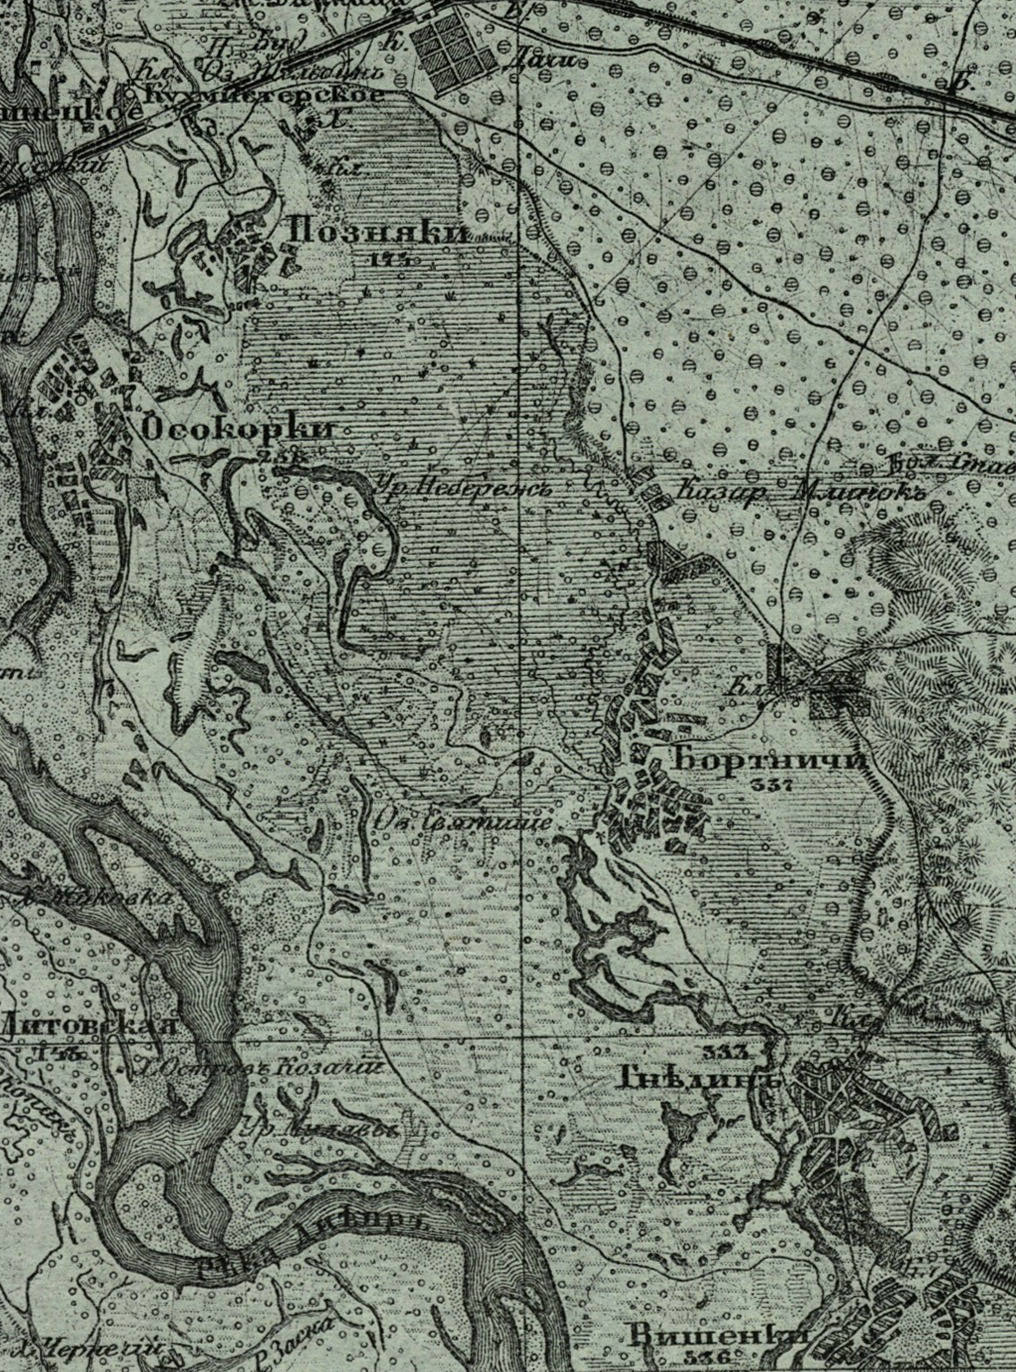
\includegraphics[width=\linewidth]{chast-gorodki/terbin/s_volocha-01.jpg}
\end{center}
\vspace*{\fill}
\newpage

Что же мы видим? У Позняков и Осокорков сам черт голову сломит. Выверты низовий Тельбина, какие-то громадные старицы у болота урочища Небреж. А вот от Бортничей начинается будто цельная река. Оттуда на юг мимо Гнедина, Вишенок.

Поглядим на лист карты Шуберта, который лежит южнее. Это лист 9, ряд XXIII. Здесь продолжается река, идущая от Бортничей вдоль Гнедина и Вишенок. В верхней правой четверти, параллельно Днепру, видно ее устье. Какая стоит подпись? «Р. Уволочье». Речка Уволочье!

\begin{center}
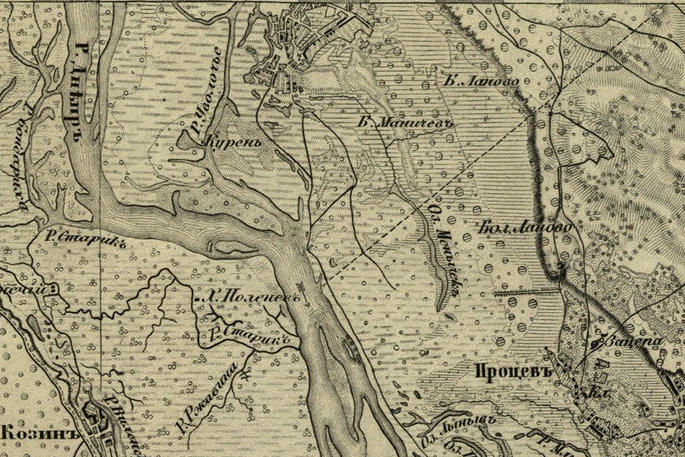
\includegraphics[width=\linewidth]{chast-gorodki/terbin/s_volocha-02.jpg}
\end{center}

Очевидно, что это – сохраненное именно старожилами название, и полагаю, что летописная «Золоча» впадала в Днепр именно здесь. Только букву «З» считаю ошибочной, ибо название Волоча оправдано волочением туда судов и прижилось в обиходе вплоть до 19 столетия, превратившись в Уволочье.

Низовье этого «Уволочья» современные уже картографы переделали в «озеро Золоче», наверное полагая, что восстанавливают историческую справедливость. Так или иначе, Волочу еще можно проследить на карте 21 века от Бортничей и на юг. Судя по имени одного из озер около Бортничей – Млынного – на этой части Волочи стояла водная мельница.

Мне остается в этой главе попробовать объяснить название Долобского и его производного – Тельбина.

В летописи есть рассказ о народе Дулебов:

\begin{quotation}
си бо Угри почаша быти при Ираклии цари, иже ходиша на Хоздроя царя Перьскаго.

В си же времена бысть и Обре, иже воеваша на царя Ираклия и мало его не яша; си же Обри воеваша на Словены и примучиша Дулебы, сущая Словены, и насилье творях женам Дулебским: аще поехати бяше Обрину, не дадяше въпрячи коня, ни волу, но веляше въпрячи 3, или 4, или 5 жен в телегу и повести Обрина; и тако мучаху Дулебы.

Бе бо Обри телом велици, а умом горди, и потреби я Бог, и помроша вси, и не оста ни един Обрин; и есть притча в Руси и до сего дни: погибоша аки Обри; их же несть ни племени, ни наследка.
\end{quotation} 

Возможно, летописное озеро «Дулебское», ставшее потом Долобским, как-то связано с этими Дулебами.
